\documentclass{proc}

\usepackage[margin=1in]{geometry}
\usepackage{multirow}
\usepackage{graphicx}
\graphicspath{{12_graphics}}

\usepackage{caption,subcaption}

\title{More on Tables and Graphics}
\author{Anuj Nair}
\date{}

\begin{document}
\maketitle

\section{Introduction}
 Here we'll look at more tables and graphics formatting.
	\subsection{More on Tables}

			Table~\ref{tab:wrapping} uses text wrapping in the last column.
			\begin{table}[htbp]
				\caption{default}
				\begin{center}
					\begin{tabular}{| l | l | p{3cm} |}		
						\hline
						CS101 & Java & Programming with Java \\
						CS201 & Languages & Programming with language principles \\
						CS301 & Compiler & Principles of complier design and implementation \\
						\hline
					\end{tabular}
				\end{center}
				\label{tab:wrapping}
			\end{table}
			

			Table~\ref{tab:multi} uses row and column span.
			\begin{table}[htbp]
				\caption{Spanning rows and columns}
				\begin{center}
					\begin{tabular}{| l | c | c |}		
						\hline
						& \multicolumn{2}{c|}{Ranges}\\
						\cline{2-3}
						& X & Y \\
						\hline
						\multirow{3}{*}{Hot}& 7 & 9\\
																& 5 & 6 \\
																& 6 & 7\\
																\hline
						\multirow{3}{*}{Cold}& 4 & 7\\
																& 2 & 9 \\
																& 3 & 5 \\
						\hline
					\end{tabular}
				\end{center}
				\label{tab:multi}
			\end{table}
   
				\subsection{More on Graphics}
				Both of my graphics are in the graphics folder for the subfigures, Figure~\ref{fig:paper} and Figure~\ref{fig:page} in Figure~\ref{fig:subs}.			
			
							  \begin{figure}[htbp]
									\centering
										\begin{subfigure}[b]{0.2\textwidth}
													\centering
													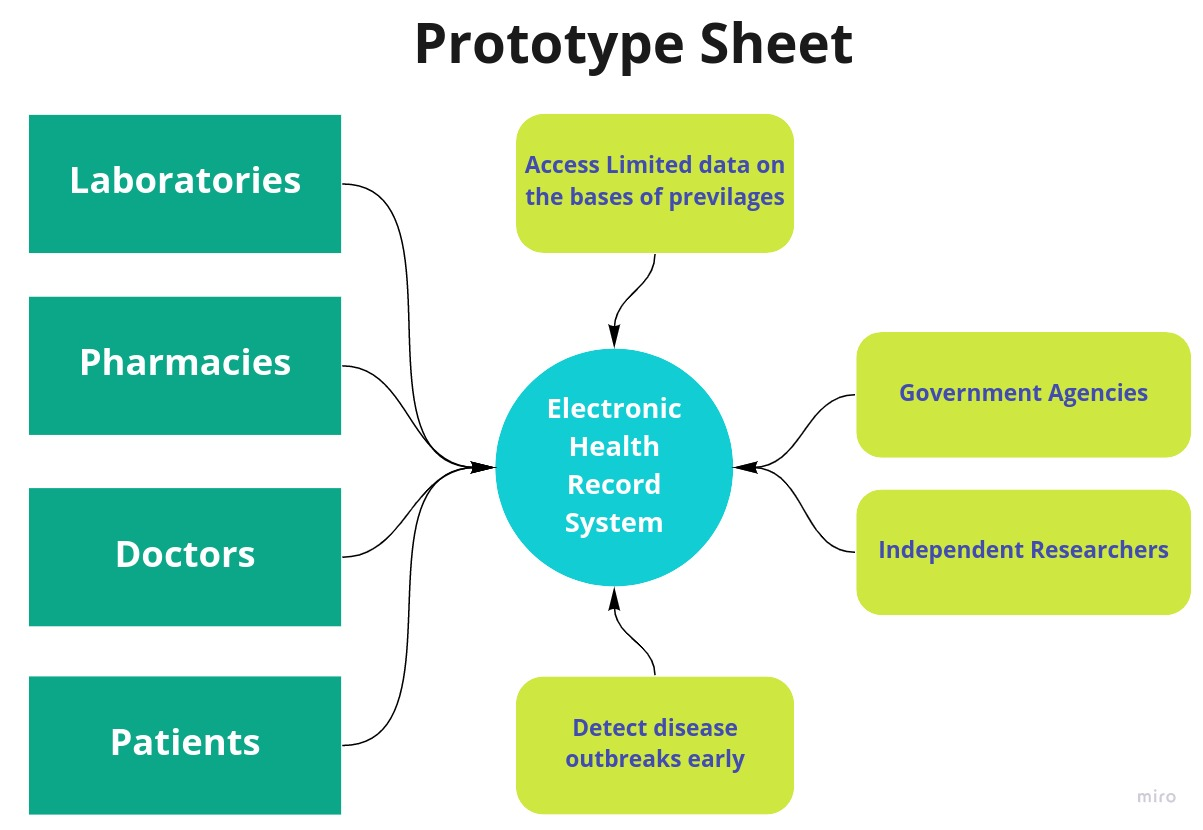
\includegraphics[scale=0.05]{protoypeSheet.jpg}
													\caption{Beginning}
													\label{fig:paper}
										\end{subfigure}%
											\begin{subfigure}[b]{0.2\textwidth}
													\centering
													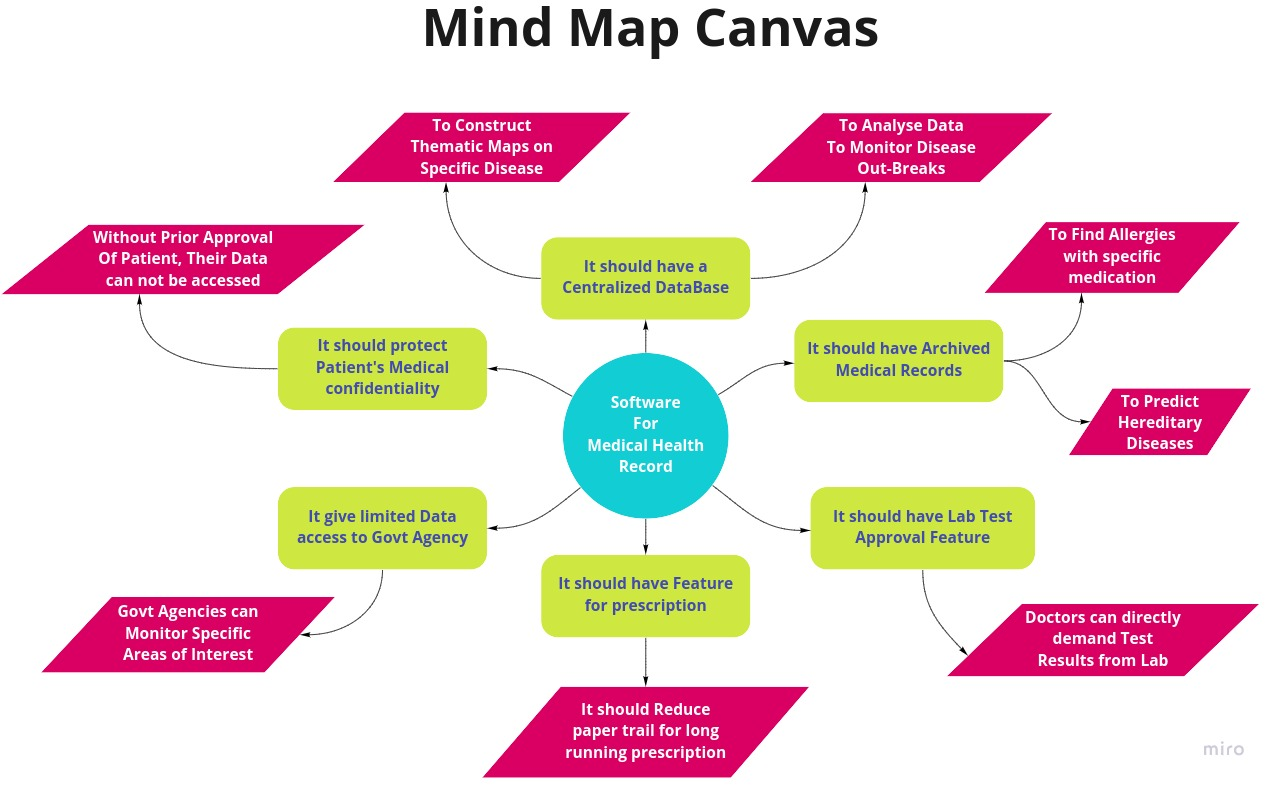
\includegraphics[scale=0.05]{MindMap2.jpg}
													\caption{End}
													\label{fig:page}
											\end{subfigure}%
												
									\caption{The process}
									\label{fig:subs}
								\end{figure}
 
				

\section{Conclusion}

 Now I know more about tables and graphics.


\end{document}
